\newcommand{\lecturetitle}[1]{
  \title{01204211 Discrete Mathematics \\ #1}
  \author{Jittat Fakcharoenphol}
  \frame{\titlepage}
}
\newcommand{\Mod}{\,\bmod\,}

\lecturetitle{Lecture 10a: Applications} 

\begin{frame}
  \frametitle{Factory Production}

  A food factory can produce 2 products: a sleeping candy bar ($S$)
  and an energy bar ($E$).

  \begin{itemize}
  \item
    There are two ingredients: $A$ and $B$.  The factory has $120$
    units of $A$ and $100$ units of $B$.
  \item
    To produce $1$ unit of candy bar $S$, you need $15$ units of $A$
    and $10$ units of $B$.
  \item
    To produce $1$ unit of energy bar $E$, you need $10$ units of $A$
    and $20$ units of $B$.
  \end{itemize}

  \pause

  How can we visualize the problem?
\end{frame}

\begin{frame}
  \frametitle{Factory Production}

  {\tiny
  A food factory can produce 2 products: a sleeping candy bar ($C$)
  and an energy bar ($E$).

  \begin{itemize}
  \item
    There are two ingredients: $A$ and $B$.  The factory has $120$
    units of $A$ and $100$ units of $B$.
  \item
    To produce $1$ unit of candy bar $C$, you need $15$ units of $A$
    and $10$ units of $B$.
  \item
    To produce $1$ unit of energy bar $E$, you need $10$ units of $A$
    and $20$ units of $B$.
  \end{itemize}

  How can we visualize the problem?
  }

  \begin{center}
    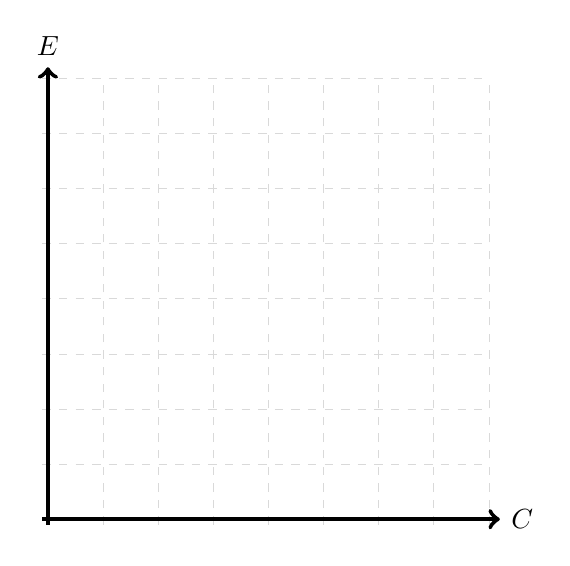
\begin{tikzpicture}[scale=0.7]
      \draw[help lines, color=gray!30, dashed] (-0.1,-0.1) grid (8,8);
      \draw[->,ultra thick] (-0.1,0)--(8.2,0) node[right]{$C$};
      \draw[->,ultra thick] (0,-0.1)--(0,8.2) node[above]{$E$};
    \end{tikzpicture}
  \end{center}
\end{frame}

\begin{frame}
  \frametitle{Factory Production}

  How can we choose the amount of $C$ and $E$ to produce?
  \pause

  It depends on the prices per unit of $C$ and $E$. \pause

  What if $1$ unit of $C$ is $1$ baht and $1$ unit of $E$ is also $1$ baht?

  \begin{center}
    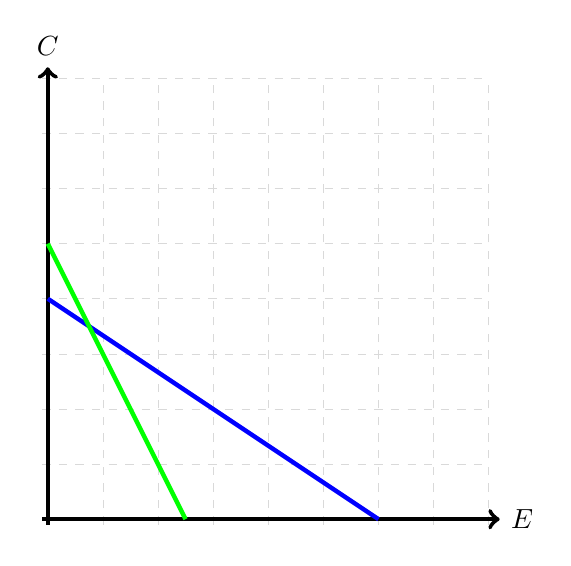
\begin{tikzpicture}[scale=0.7]
      \draw[help lines, color=gray!30, dashed] (-0.1,-0.1) grid (8,8);
      \draw[->,ultra thick] (-0.1,0)--(8.2,0) node[right]{$E$};
      \draw[->,ultra thick] (0,-0.1)--(0,8.2) node[above]{$C$};

      \draw[ultra thick, blue] (0,4)--(6,0);
      \draw[ultra thick, green] (0,5)--(2.5,0);
    \end{tikzpicture}
  \end{center}
\end{frame}

\begin{frame}
  \frametitle{Factory Production}

  How can we choose the amount of $C$ and $E$ to produce?
  \pause

  It depends on the prices per unit of $C$ and $E$. \pause

  What if $1$ unit of $C$ is $1$ baht and $1$ unit of $E$ is also $1$ baht?

  \begin{center}
    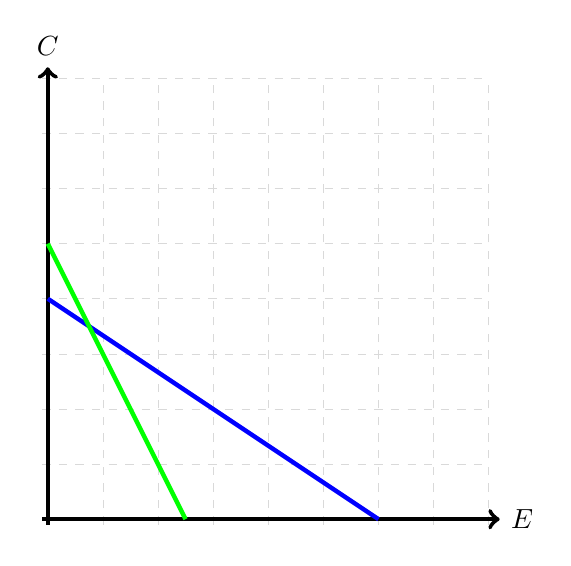
\begin{tikzpicture}[scale=0.7]
      \draw[help lines, color=gray!30, dashed] (-0.1,-0.1) grid (8,8);
      \draw[->,ultra thick] (-0.1,0)--(8.2,0) node[right]{$E$};
      \draw[->,ultra thick] (0,-0.1)--(0,8.2) node[above]{$C$};

      \draw[ultra thick, blue] (0,4)--(6,0);
      \draw[ultra thick, green] (0,5)--(2.5,0);
    \end{tikzpicture}
  \end{center}
\end{frame}

\begin{frame}
  \frametitle{Factory Production}

  What if $1$ unit of $C$ is $10$ baht and $1$ unit of $E$ is also $1$ baht?

  \begin{center}
    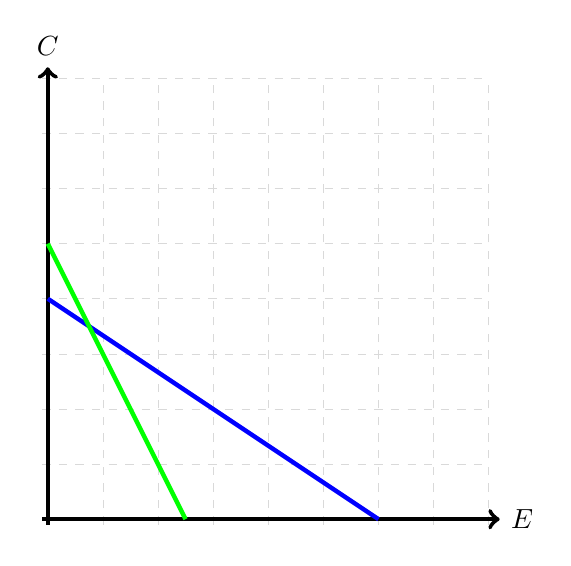
\begin{tikzpicture}[scale=0.7]
      \draw[help lines, color=gray!30, dashed] (-0.1,-0.1) grid (8,8);
      \draw[->,ultra thick] (-0.1,0)--(8.2,0) node[right]{$E$};
      \draw[->,ultra thick] (0,-0.1)--(0,8.2) node[above]{$C$};

      \draw[ultra thick, blue] (0,4)--(6,0);
      \draw[ultra thick, green] (0,5)--(2.5,0);
    \end{tikzpicture}
  \end{center}
\end{frame}

\begin{frame}
  \frametitle{Factory Production}

  What if $1$ unit of $C$ is $1$ baht and $1$ unit of $E$ is also $10$ baht?

  \begin{center}
    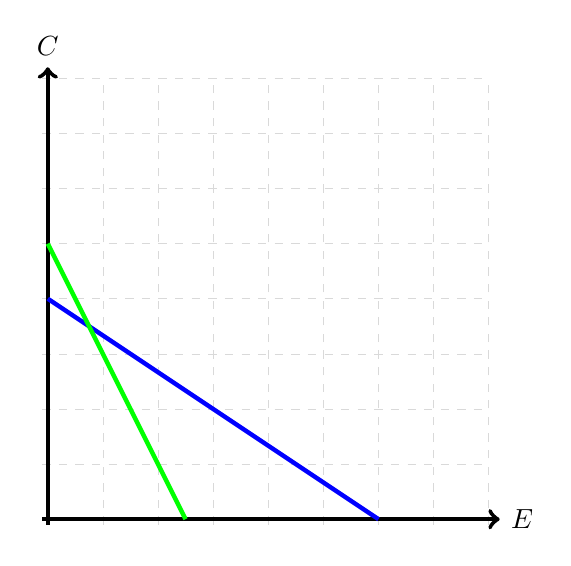
\begin{tikzpicture}[scale=0.7]
      \draw[help lines, color=gray!30, dashed] (-0.1,-0.1) grid (8,8);
      \draw[->,ultra thick] (-0.1,0)--(8.2,0) node[right]{$E$};
      \draw[->,ultra thick] (0,-0.1)--(0,8.2) node[above]{$C$};

      \draw[ultra thick, blue] (0,4)--(6,0);
      \draw[ultra thick, green] (0,5)--(2.5,0);
    \end{tikzpicture}
  \end{center}
\end{frame}

\begin{frame}
  \frametitle{Objective functions}

  If we produce $x_1$ units of $C$ and $x_2$ units of $E$, we would make
  \pause
  \[
  p_C\cdot x_1 + p_E\cdot x_2,
  \]
  where $p_C$ and $p_E$ are unit prices for $C$ and $E$.
  \pause
  
  This is called an objective function.  So far, we tried 3 objective functions:
  \begin{itemize}
  \item $x_1+x_2$
  \item $10\cdot x_1 + x_2$
  \item $x_1 + 10\cdot x_2$
  \end{itemize}

\end{frame}

\begin{frame}
  \frametitle{Objective functions}

  Let's see what they look like again. 
  
  \begin{center}
    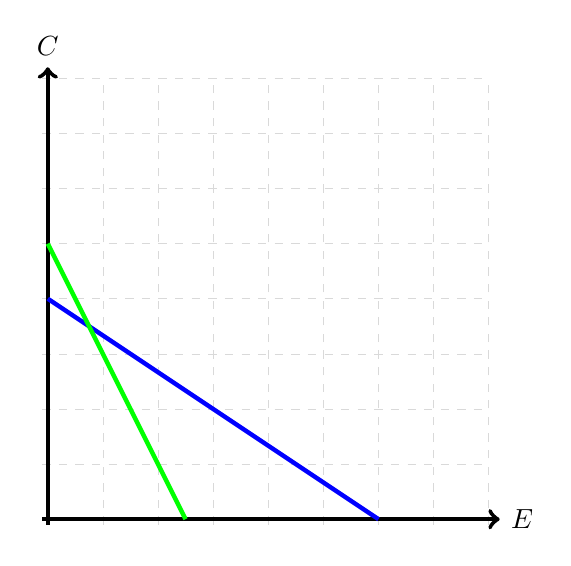
\begin{tikzpicture}[scale=0.7]
      \draw[help lines, color=gray!30, dashed] (-0.1,-0.1) grid (8,8);
      \draw[->,ultra thick] (-0.1,0)--(8.2,0) node[right]{$E$};
      \draw[->,ultra thick] (0,-0.1)--(0,8.2) node[above]{$C$};

      \draw[ultra thick, blue] (0,4)--(6,0);
      \draw[ultra thick, green] (0,5)--(2.5,0);
    \end{tikzpicture}
  \end{center}
\end{frame}

\begin{frame}
  \frametitle{Vertices}

  Interesting things happen at the intersections.  What are they?
  
  \begin{center}
    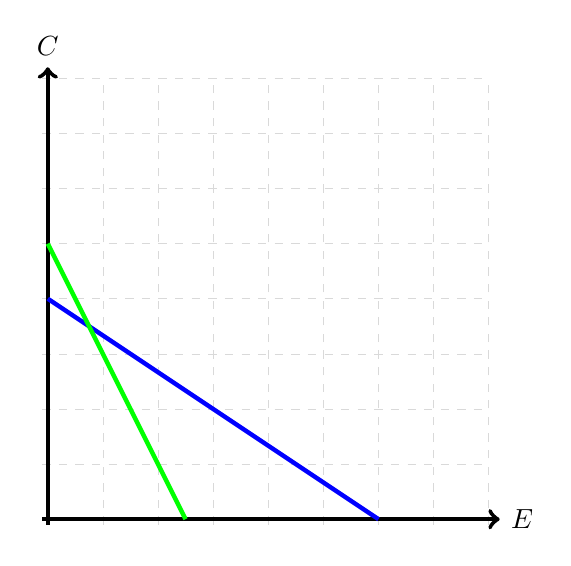
\begin{tikzpicture}[scale=0.7]
      \draw[help lines, color=gray!30, dashed] (-0.1,-0.1) grid (8,8);
      \draw[->,ultra thick] (-0.1,0)--(8.2,0) node[right]{$E$};
      \draw[->,ultra thick] (0,-0.1)--(0,8.2) node[above]{$C$};

      \draw[ultra thick, blue] (0,4)--(6,0);
      \draw[ultra thick, green] (0,5)--(2.5,0);
    \end{tikzpicture}
  \end{center}
\end{frame}

\begin{frame}
  \frametitle{Simplex algorithm}
  \begin{center}
    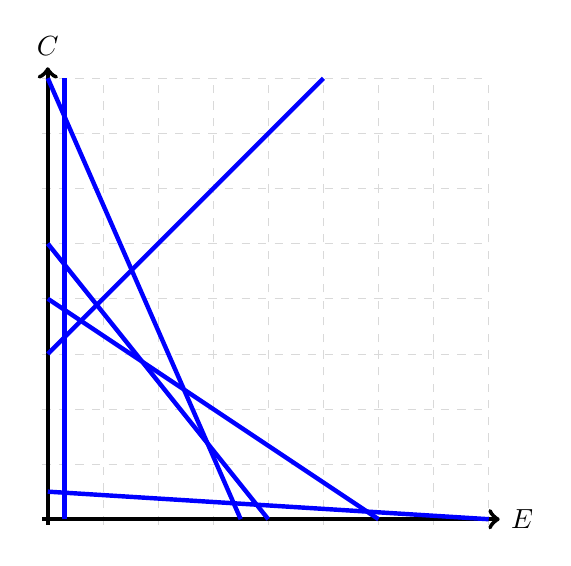
\begin{tikzpicture}[scale=0.7]
      \draw[help lines, color=gray!30, dashed] (-0.1,-0.1) grid (8,8);
      \draw[->,ultra thick] (-0.1,0)--(8.2,0) node[right]{$E$};
      \draw[->,ultra thick] (0,-0.1)--(0,8.2) node[above]{$C$};

      \draw[ultra thick, blue] (0,0.5)--(8,0);
      \draw[ultra thick, blue] (0.3,0)--(0.3,8);
      \draw[ultra thick, blue] (0,4)--(6,0);
      \draw[ultra thick, blue] (0,8)--(3.5,0);
      \draw[ultra thick, blue] (0,5)--(4,0);
      \draw[ultra thick, blue] (0,3)--(5,8);
    \end{tikzpicture}
  \end{center}
\end{frame}

\begin{frame}
  \frametitle{Simplex algorithm - How do you move?}
  \begin{center}
    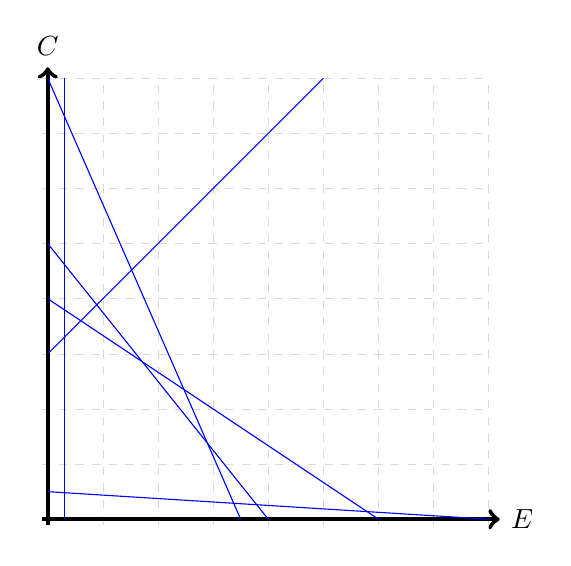
\begin{tikzpicture}[scale=0.7]
      \draw[help lines, color=gray!30, dashed] (-0.1,-0.1) grid (8,8);
      \draw[->,ultra thick] (-0.1,0)--(8.2,0) node[right]{$E$};
      \draw[->,ultra thick] (0,-0.1)--(0,8.2) node[above]{$C$};

      \draw[blue] (0,0.5)--(8,0);
      \draw[blue] (0.3,0)--(0.3,8);
      \draw[blue] (0,4)--(6,0);
      \draw[blue] (0,8)--(3.5,0);
      \draw[blue] (0,5)--(4,0);
      \draw[blue] (0,3)--(5,8);
    \end{tikzpicture}
  \end{center}
\end{frame}

\begin{frame}
  \frametitle{A quick history of machine learning}
  \begin{itemize}
  \item Perceptrons
  \item Neural networks
  \item Convolutional neural networks
  \end{itemize}
\end{frame}

\begin{frame}
  \frametitle{Perceptrons}
  {
    \small
    \begin{itemize}
    \item Invented in 1943 by McCulloch and Pitts.
    \item Implemented by Rosenblatt in 1958 (The Perceptron algorithm).
    \end{itemize}
  }
  \vspace{2.5in}
\end{frame}

\begin{frame}
  \frametitle{Perceptrons: Training the weights}
\end{frame}

\begin{frame}
  \frametitle{Perceptrons: XOR limit and multilayer perceptrons}
\end{frame}

\begin{frame}
  \frametitle{Neural networks}
\end{frame}

\begin{frame}
  \frametitle{Inspiration from visual cortex study}
\end{frame}

\begin{frame}
  \frametitle{Convolutional neural networks}
\end{frame}
